% Chapter 4

\chapter{Results} % Chapter title

\label{ch:results} % For referencing the chapter elsewhere, use \autoref{ch:introduction} 

%----------------------------------------------------------------------------------------
\section{List of Sources}
Twenty three sources were analysed; a full list is shown below:
\begin{itemize}
\item 1A0535+262
\item AXJ1910.7+0917
\item Cen X-3
\item EXO2030+375
\item IGRJ08408-4503
\item IGRJ11215-5952
\item IGRJ16418-4532
\item IGRJ16465-4507
\item IGRJ16479-4514
\item IGRJ17391-3021
\item IGRJ17407-2808
\item IGRJ17544-2619
\item IGRJ18027-2016
\item IGRJ18219-1347
\item IGRJ18410-0535
\item IGRJ18450-0435
\item IGRJ18483-0311
\item MAXIJ1409-619
\item OAO1657-415
\item SAXJ1818.6-1703
\item SMCX-1
\item Vela X-1
\item XPer
\end{itemize}
\clearpage{}

\section{Cen X-3}

\begin{figure}[h!]
\centering
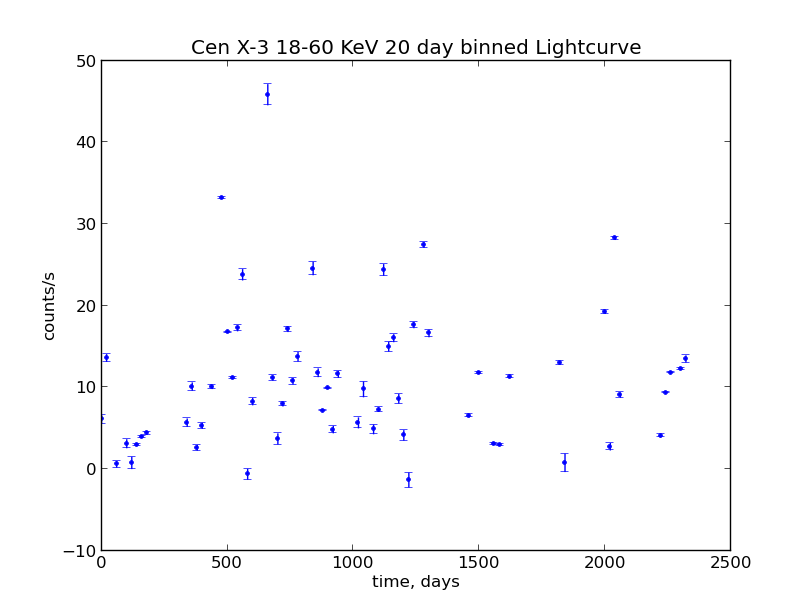
\includegraphics[width=130mm]{gfx/Fig7.png}
\caption{20 day binned lightcurve for Cen X-3.}
\label{Figure 7}
\end{figure}

Cen X-3 is a very bright and well studied source, and as it\textquoteright{}s designation would suggest, was one of the first X-ray sources to be discovered. It is a SGXB, and so is powered primarily by stellar wind loss. It has a well documented 2.087 day cycle.

\begin{figure}[h!]
\centering
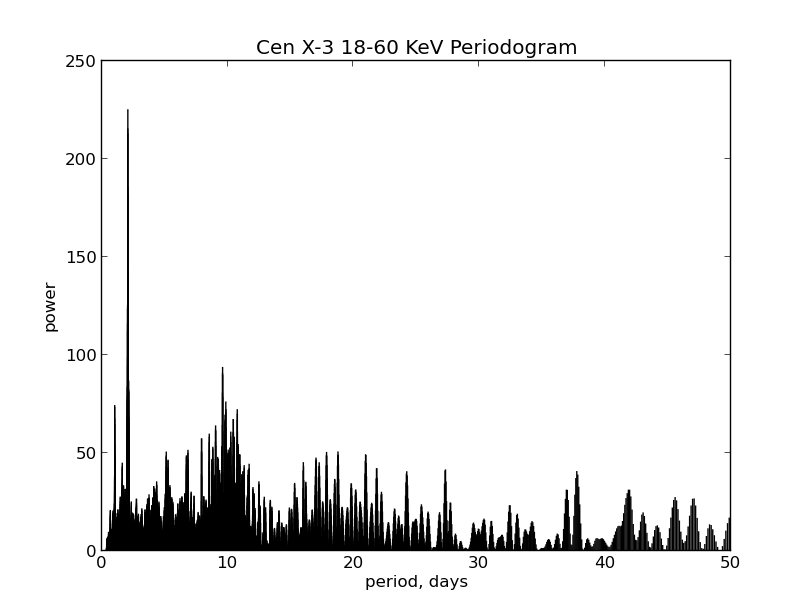
\includegraphics[width=130mm]{gfx/Fig8.png}
\caption{Periodogram for Cen X-3. The expected peak at 2.087 days is very clear.}
\label{Figure 8}
\end{figure}

\ref{Figure 9} shows a binned lightcurve. Although this does not reveal anything useful, it is an example of a particularly good source. Cen X-3 is very luminous, and the error bars and count rates reflect this. \ref{Figure 8} shows a periodogram from Cen X-3. The expected peak at 2.087 days is very clear. Once folded on this period, \ref{Figure 9} shows the eclipse profile. From these results, it is easy to see that Cen X-3 shows the behaviour expected of a SGXB. It is luminous and active except when eclipsing, and provides a good example to measure other less well known and more uncertain sources against. 

\begin{figure}[h!]
\centering
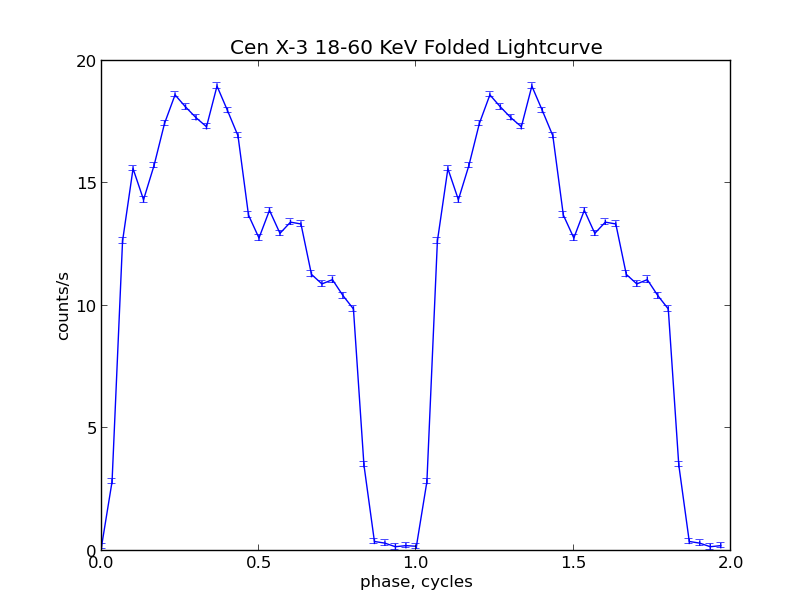
\includegraphics[width=130mm]{gfx/Fig9.png}
\caption{Folded lightcurve for Cen X-3.}
\label{Figure 9}
\end{figure} 

\clearpage
\section{}